\documentclass[12pt,a4paper]{article}
\usepackage[utf8]{inputenc}
\usepackage[english]{babel}
\usepackage{setspace}
\usepackage{geometry}
\usepackage{graphicx}
\usepackage{caption}
\usepackage{hyperref}

\newgeometry{left=1in, top=1in, bottom=1in, right=1.5in}

\title{Space Debris Clustering}
\author{Daniel Kolosa}
\date{04-27-2017}

\doublespacing

\begin{document}
\maketitle

\section{Introduction}
This project clusters a portion of debris orbiting Earth. The first section is background material on what is space debris and why is it an issue. The second section describes the dataset that is used for the statistical models used. The third section will discus the statistical models and their results. The final section is the conclusion and any possible future work.   

\section{Background}
Ever since humans have been sending things into space we have not been cleaning up after ourselves. The debris that is in space are remains of dead satellites, rocket chassis, engines, components of space stations, and other miscellaneous items. Fortunately, some items that are close enough to Earth reenter the atmosphere are burn up on reentry, but there are still many objects that will remain in orbit for many years. The objects that will remain in orbit travel at very high speeds and can cause millions of dollars of damage if they collide with working space vehicles, or generate more debris if they collide with other objects. Also if the number of space debris continues to increase, than space exploration may not become possible due to the risk of damage from the large amount of debris. The dataset used is a collection of objects orbiting in the Low-Earth orbit (LEO) region. There are many other regions including, Geo-synchronous orbit (GEO), high earth orbit (HEO) but LEO orbit has a majority of debris and other objects. 

\section{Dataset}
%Satellite tracking data is encoded in a two line element set. The two line element set encodes position and velocity of a satellite based on its orbital elements. Orbital elements is a coordinate system used to describe the shape of an orbit. The two element set also includes data such as identification number, security classification either classified or unclassified epoch lauch dates, and atmospheric drag coefficients. The position and velocity of the objects are computed using simplified pertubation models. The simplified pertubation models are used to compute the orbital state of an object which taking into account the shape of the Earth, radiation, atmospheric drag, and gravitional influence from the Moon and Sun.

The dataset used for this project is provided by space-track.org. This organization collects and maintains datasets of satellite position status and position data. The observations in this dataset contain both debris and operational vehicles. The data is obtained from NORAD(North American Aerospace Defense Command) and NASA. The objects in this dataset are: debris, payload, rocket bodies, and others. Debris in this context consists of satellite and spacecraft fragments, payload is made up of capsules of supplies or satellites. Rocket bodies consist of discarded rockets that were used to launch objects into orbit. The figure below shows what kind of objects and how many objects are in each category.
\begin{center}
	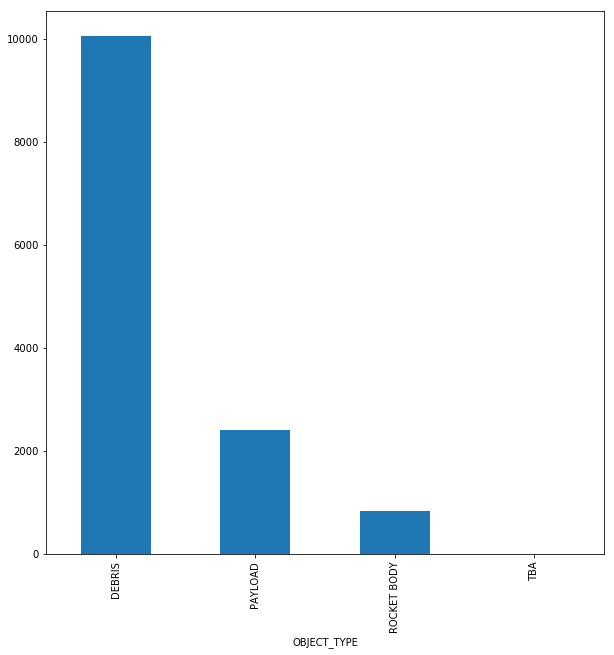
\includegraphics[scale=0.25]{figures/object_types.png}
	\captionof{figure}{Distribution of object size}
	\label{fig:object_types}
\end{center}
It can be seen from the figure above, that debris make up a significant amount of objects of the dataset. 

Along with the object type the radar cross-section is an important metric to look at. The radar cross section is used to estimate the cross-sectional area of an object. Specific values for the radar cross section is not provided due to security reasons or lack of accuracy from the ground station sensors. Radar cross section is divided into three categories, small, medium, and large. Small are objects <$.1 m^2$, medium are objects between .1$m^2$ and 1$m^2$, and large objects are > $1m^2$\cite{spaceTrack}.

The plot below shows the number of objects for the three different sizes.
\begin{center}
	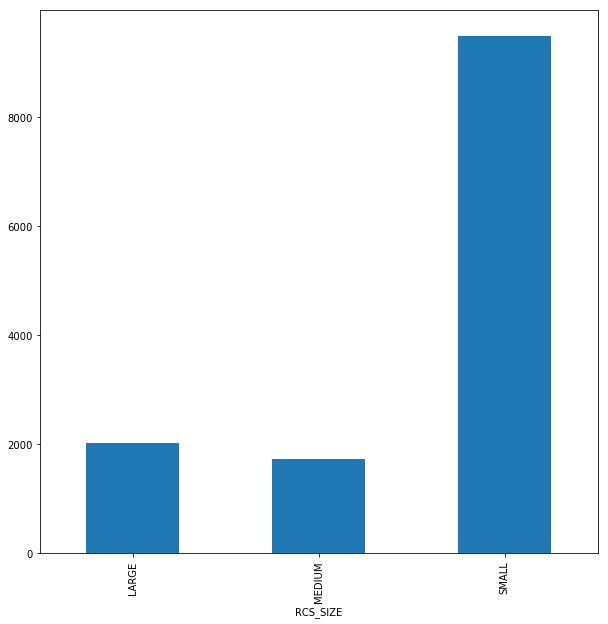
\includegraphics[scale=0.25]{figures/RCS_size.png}
	\captionof{figure}{Number of objects by object type}
	\label{fig:RCS_size}
\end{center}
Looking at the plot above, it can be seen that the most objects in the dataset have a small cross section. This gives a good visualization of what kind of debris are in orbit.

The given dataset also provides orbital element data. The orbital element data provided are: apogee, perigee, inclination, and Period. The apogee and perigee are the maximum and minimum radii of an elliptical orbit, respectively. The inclination is the tilt angle of the orbit relative to the Earth's equator and the period is the time it takes for the object to orbit the Earth in one revolution. 

The dataset must go through some preprocessing before it can be used. The velocity can be approximated as the mean orbit speed from the equations below\cite{Curtis}.
\begin{equation}
\begin{matrix}
v = \frac{2a}{T} \quad a = \frac{r_p + r_a }{2}
\end{matrix}
\end{equation}
where T is the orbit period given by the dataset in minutes and a is the semi-major axis in kilometers, and $r_p$ and $r_a$ are the perigee and apogee radii, respectively

The data must be converted into numeric data for a classifier to use. Using one-hot encoding, a matrix is created to represent the sizes of the objects.

\section{Statistical Model and Results}
This dataset does not 
Since the dataset will be analyzed with unsupervised learning techniques, K-means clustering and a dendrogram will be used. The features that will be analyzed is radar cross section sizes and mean orbit speed. These features were selected because for this study finding a subgroup or correlation between the size of an object and its speed can give an insight into how much risk it can pose to operational space vehicles.   For these methods to work, the radar cross section sizes must be converted into numeric data for a classifier to use. Using one-hot encoding, a matrix is created to represent the sizes of the objects.  The number of clusters for the k-means classification is selected by measuring the disturbance at different values of clusters.
\begin{center}
	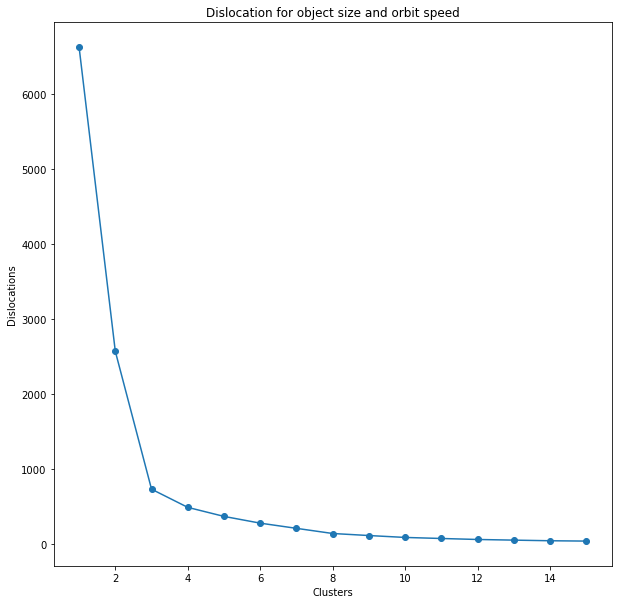
\includegraphics[scale=0.25]{figures/dislocation_obj_size.png}
	\captionof{figure}{Elbow Plot}
	\label{fig:Dislocation}
\end{center}
As seen in the figure above, using three or four clusters would be a good start for this situation. Using four clusters, a silhouette analysis is done. The silhouette plot will give an idea of the separation distance between the clusters.

\begin{center}
	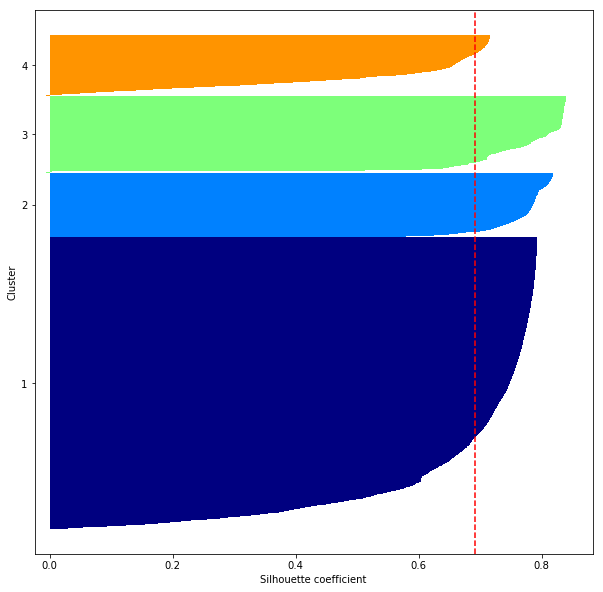
\includegraphics[scale=0.25]{figures/Silhouette.png}
	\captionof{figure}{Silhouette Analysis}
	\label{fig:Silhouette}
\end{center}

The Silhouette plot above shows a mean silhouette coefficient of 0.7 which is good degree of separation, also with four clusters there is not much improvement in the silhouette coefficient, so in this case, using three clusters would be optimal.
The final method that will be looked at is a dendrogram plot. A dendrogram plot shows the correlation between clusters in a dataset.
\begin{center}
	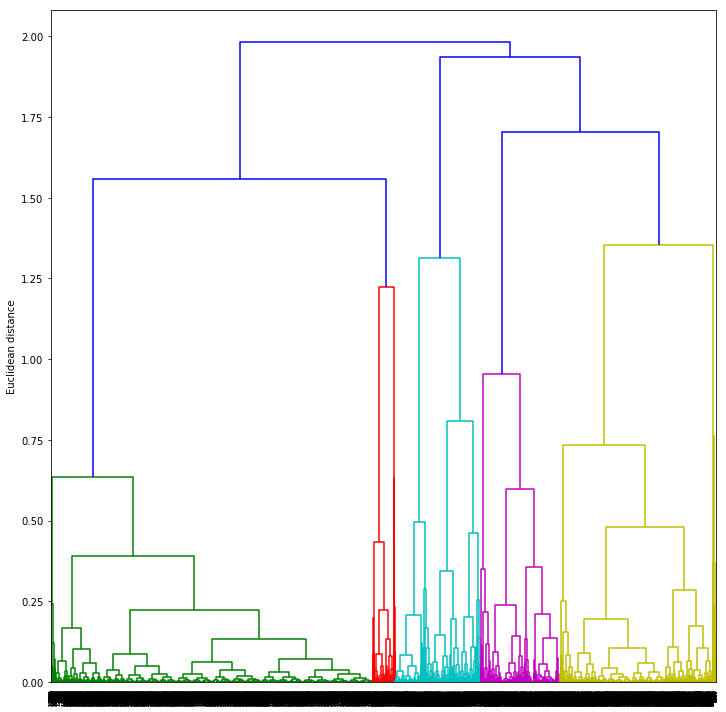
\includegraphics[scale=0.3]{figures/dendrogram.png}
	\captionof{figure}{dendrogram plot}
	\label{fig:dendrogram}
\end{center}
The dendrogram above, shows that a horizontal cut can be made at 1.5 giving five different clusters. Looking at the Euclidean distances, between the clusters there is little correlation between the clusters.  Looking at both the dendrogram and silhouette plots, there are no negative values meaning that there are no negative correlations. Clustering other features like radar cross section size and object type were looked at but gave many misclassification.
\section{Conclusion}
This paper goes into the background information on space debris including the dangers and importance. Then the dataset was introduced and the preprocessing methods. A k-means classifier was analyzed using an elbow and a silhouette plot and a dendrogram was created to show the relationship of the clusters.

The future work of this project could include implementing more complicated models like using neural networks. Also it would be interesting to introduce drag models and get quantitative data on the size and create predictive risk assessment model.

\begin{thebibliography}{5}
\bibitem{spaceTrack} \url{space-track.org}
\bibitem{Curtis} Curtis, H., D., "Orbital Mechanics for Engineering Students", Ed.1, Elsevier Butterworth-Heinemann, January 10, 2005
\end{thebibliography}
 
\end{document}
